\documentclass[11pt]{article}

\usepackage{amssymb,amsmath,amsfonts,eurosym,geometry,ulem,graphicx,caption,color,setspace,sectsty,comment,footmisc,caption,natbib,pdflscape,subfigure,array,hyperref}
\hypersetup{unicode=true}

\normalem

\singlespacing
\newtheorem{theorem}{Theorem}
\newtheorem{corollary}[theorem]{Corollary}
\newtheorem{proposition}{Proposition}
\newenvironment{proof}[1][Proof]{\noindent\textbf{#1.} }{\ \rule{0.5em}{0.5em}}

\newtheorem{hyp}{Hypothesis}
\newtheorem{subhyp}{Hypothesis}[hyp]
\renewcommand{\thesubhyp}{\thehyp\alph{subhyp}}

\newcommand{\red}[1]{{\color{red} #1}}
\newcommand{\blue}[1]{{\color{blue} #1}}

\newcolumntype{L}[1]{>{\raggedright\let\newline\\arraybackslash\hspace{0pt}}m{#1}}
\newcolumntype{C}[1]{>{\centering\let\newline\\arraybackslash\hspace{0pt}}m{#1}}
\newcolumntype{R}[1]{>{\raggedleft\let\newline\\arraybackslash\hspace{0pt}}m{#1}}

\geometry{left=1.0in,right=1.0in,top=1.0in,bottom=1.0in}

\begin{document}

\begin{titlepage}
\title{Placeholder\thanks{abc}}
\author{Hyunwoo Park\thanks{abc} \and John Smith\thanks{abc}}
\date{\today}
\maketitle
\begin{abstract}
\noindent Placeholder\\
\vspace{0in}\\
\noindent\textbf{Keywords:} key1, key2, key3\\
\vspace{0in}\\
\noindent\textbf{JEL Codes:} key1, key2, key3\\

\bigskip
\end{abstract}
\setcounter{page}{0}
\thispagestyle{empty}
\end{titlepage}
\pagebreak \newpage

\singlespacing


\section{Introduction} \label{sec:introduction}

\section{Literature Review} \label{sec:literature}

\section{Data} \label{sec:data}

\section{Results} \label{sec:result}

\section{Discussions} \label{sec:discussion}

\section{Conclusion} \label{sec:conclusion}



\singlespacing
\setlength\bibsep{0pt}
\bibliographystyle{apalike}
\bibliography{/Users/aassumpcao/library.bib}

\clearpage

\singlespacing

\section*{Tables} \label{sec:tab}

\clearpage

\section*{Figures} \label{sec:fig}

%\begin{figure}[hp]
%  \centering
%  \includegraphics[width=.6\textwidth]{../fig/placeholder.pdf}
%  \caption{Placeholder}
%  \label{fig:placeholder}
%\end{figure}


\clearpage

\section*{Appendix A: Service Order Classification} \label{sec:appendixa}

Service orders issued by CGU investigated different uses of public resources in addition to procurement, e.g.~for officials compensation, for school activities, or for community monitoring of public policies. The discretion measure proposed here, however, is exclusive to procurement expenditures made under Law 8,666/93. The ideal dataset for this study would contain explicit procurement information collected by CGU auditors, but unfortunately this is not the case. The reporting of procurement processes is implicit, via descriptions of investigations or findings of violations to Law 8,666/93. Thus, we isolate service orders which investigated procurement processes from the rest by implementing an classification system based on the information retrieval and natural-language processing literatures.

The system uses each service order's description to identify if it is procurement-related. In these descriptions, CGU auditors report the purpose of their investigation, e.g.~whether they are looking into painkiller purchases, whether the municipality has used the funds within designated goals, or whether primary school teachers were hired for the implementation of a school program. Using these textual descriptions as bag-of-words models, we implement a method similar to that of \citet{HopkinsMethodAutomatedNonparametric2009}: we stem and combine unigrams to form search patterns that identify a service order as procurement-related. There are two broad types of procurement in Law 8,666/93: (i) ordinary procurement of goods and services, which we call \emph{purchases}; and (ii) procurement of goods and services used for public works, which we call \emph{works}. There are different search patterns for each type.

An example is useful for understanding our classification process. Unigram ``aquisição'' (\emph{acquisition} in English) is stemmed to ``aquisi'' to form a search pattern for the \emph{purchases}-type procurement; unigrams ``adequação'' and ``habitacional'' are stemmed and combined to form ``adequa(.)*habitac''\footnote{All seach patterns are   regular expressions.} search pattern for \emph{works}-type procurement. This bigram picks up variations in main keywords as well as coding mistakes due to, for instance, multiple whitespace between the two unigrams or due to coding Portuguese special characters (``adequação'' vs. ``adequacao'').

\begin{table}[htbp]
  \caption{\label{tab:searchterms} Procurement Search Terms}
  \centering

  \begin{tabular}{l p{.85\textwidth}}
  \hline

  \hline
  Type & Search Terms \\
  \hline
  Purchases & ``aquisi'' ``execu'' ``equipame'' ``ve{[}íi{]}culo'' ``despesa'' ``aplica{[}çc{]}'' ``medicamento(.)*peaf'' ``compra'' ``recurso(.)*financ'' ``unidade(.)*m{[}óo{]}ve(.)*sa{[}úu{]}de'' ``pnate'' ``transporte(.)*escola'' ``desenv(.)*ensino'' ``kit'' ``siafi'' ``implementa{[}çc{]}'' ``adquir'' ``pme(.)*2004'' ``aparelhamento'' \\
  \hline
  Works & ``co(ns\textbar{}sn)tru'' ``obra'' ``implant'' ``infra(.)*estrut'' ``amplia'' ``abasteci(.)*d(.)*{[}áa{]}gua'' ``reforma'' ``(melhoria\textbar{}adequa)+(.)*(f{[}íi{]}sica\textbar{}escolar\textbar{}habitac\textbar{}sanit{[}áa{]}ria)+'' ``esgot'' ``adutora\textbar{}dessaliniz\textbar{}reservat{[}óo{]}'' ``sanit{[}áa{]}ri{[}ao{]}'' ``poço'' ``aperfei{[}çc{]}oa'' ``saneamento'' ``res{[}íi{]}duo(.)*s{[}óo{]}lido'' ``conclus{[}ãa{]}o''\\
  \hline

  \hline
  \end{tabular}
\end{table}

The final list contains 19 \emph{n}-grams for identification of purchases and 17 \emph{n}-grams for works.\footnote{One of these keywords in the works search pattern is an ``exclusion keyword,'' which removes service orders that contain the ``exclusion keyword'' in their description from the sample identified by the other 16 \emph{n}-grams.} When any of these words is found, we include the service order into the purchases or the works group. Since all public works projects procure goods and services but not all public purchases are works-related, whenever the search patterns matches service orders to both groups, we include the service order only in the works group but not in the purchases group. Public works procurements are a subset of all public procurements in Brazilian municipalities. The search patterns here identify a total of 9,593 procurement-related service orders.

\begin{figure}[!htbp]
{\centering 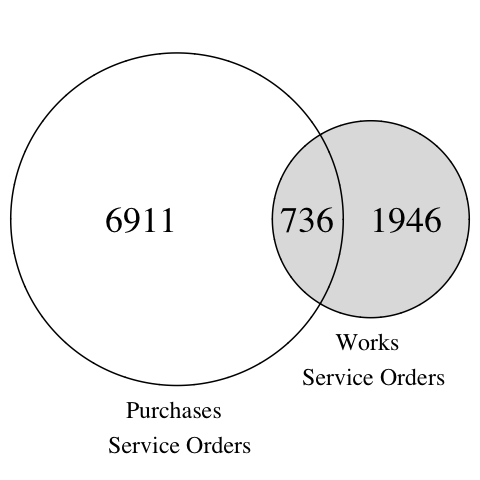
\includegraphics[width=0.3\linewidth]{venn}

}
\caption{\label{fig:venn} Sets of Procurement Service Orders}
\end{figure}

As \citet{GrimmerTextDataPromise2013a} rightly point out, no text analysis algorithm is perfect and only relying on keyword matches could potentially lead to misclassification of service orders. Let us suppose that one description reads ``expenditures made in accordance with primary education program.'' Using unigram ``expenditure'' would yield a match for this service order to the purchases group, but in fact auditors might be looking at bonus payments for high-performing teachers. These resources could also be directed for school construction. In the first case, the service order should not be have been included in any group because it does not carry any procurement component. In the second case, it should have also been marked as public works.

We address these classification problems in three ways: (i) using means comparison tests of match quality discussed in \citet{AssumpcaotextfindDataDrivenText2018}; (ii) comparing the performance of the same search patterns on another textual description for a subset of service orders; (iii) finally, comparing the results from the textual classification algorithm to that of procurement violations reported by CGU auditors. We discuss these three tests in turns in the following sections.

\subsection*{A.1 Means Tests}\label{quality1}

The first test on match quality is the means comparison test presented in \citet{AssumpcaotextfindDataDrivenText2018}, whose reasoning is simple. Increasing the number of procurement-related terms in the search pattern is not necessarily good practice as we increase the chance of misclassifying service orders as procurement when in fact they are not; words can take on different meanings depending on their contexts, so the more search terms we use the more likely type I error is. Ideally, we would want to use as few \emph{n}-grams as possible while still identifying all possible procurement matches. In order to do this, what \citet{AssumpcaotextfindDataDrivenText2018} suggests is testing match quality by incrementally comparing sample means identified by \emph{n} vs. \emph{n} - 1 keywords. This method translates into a check on whether the sample identified by one additional keyword is significantly better than the previous sample with one fewer term. The program developed by \citet{AssumpcaotextfindDataDrivenText2018} does this for us and we report the results in the tables below:

\end{document}